\documentclass{article}

\date{14 Octobre 2024}
\usepackage[nb-sem=5, auteurs={Kylian Boyet, George Ober, Felix Rondeau}]{../kholles}


\begin{document}

\maketitle

\begin{question_kholle}{Montrer qu'une combinaison linéaire de deux fonctions bornées (respectivement lipschitziennes) est bornée (resp. lipschitzienne)}
  Soit $I$ un intervalle réel.
  Soient $f$ et $g$ deux fonctions de $I$ dans $\mathbb{R}$ et $(\lambda, \mu) \in \mathbb{R}^2$.
  \begin{itemize}[label=$\lozenge$]
    \item Supposons que $f$ et $g$ sont respectivement bornées par $A$ et par $B$.
          Soit $x \in I$ fixé quelconque.
          \begin{align*}
            \Big| (\lambda.f + \mu.g)(x) \Big| & = \Big| \lambda.f(x) + \mu.g(x) \Big|                                             \\
                                               & \leqslant \big| \lambda \big|  \big|f(x)\big| + \big| \mu \big|  \big| g(x) \big| \\
                                               & \leqslant \big| \lambda \big| A + \big| \mu \big| B
          \end{align*}
          Donc $\lambda.f + \mu.g$ est bornée.
    \item Supposons que $f$ et $g$ sont respectivement $K$ et $L$ lipschitziennes.\\
          Soient $(x, y) \in I^2$ fixés quelconques.
          \begin{align*}
            \Big| (\lambda.f + \mu.g)(x) - (\lambda.f + \mu.g)(y)\Big| & = \Big| \lambda.f(x) + \mu.g(x) - \lambda.f(y) - \mu.g(y) \Big|                                   \\
                                                                       & = \Big| \lambda(f(x) - f(y)) + \mu(g(x) - g(y)) \Big|                                             \\
                                                                       & \leqslant \Big| \lambda  \Big|  \Big| f(x) - f(y) \Big| + \Big| \mu \Big|  \Big|g(x) - g(y) \Big| \\
                                                                       & \leqslant \Big| \lambda  \Big|  K \Big| x-y \Big| + \Big| \mu  \Big| L  \Big| x - y \Big|         \\
                                                                       & \leqslant (|\lambda| K + |\mu|L ) |x - y|
          \end{align*}
  \end{itemize}
\end{question_kholle}

\begin{question_kholle}{Montrer que si $f$ est impaire et bijective, alors $f^{-1}$ est aussi impaire. Donnez un/des exemples.}
  Soient $I$ et $J$ deux parties non-vides de $\R$ et $f$ une application bijective impaire de $I$ dans $J$. Notons $f^{-1}$ sa bijection réciproque.\\
  L'imparité de $f$ impose la symétrie de $I$ par rapport à l'origine. De plus, pour tout $y\in J$,
  \[
    \exists{x}\in I: f(x)=y
  \]
  donc par imparité de la fonction $f$, le domaine $I$ étant centré en $0$,
  \[
    f(-x)=-f(x)=-y
  \]
  Ainsi, $J$ est centré en $0$. On a alors, pour tout $y\in J$,
  \begin{align*}
    f^{-1}(-y) & = f^{-1}(-f(f^{-1}(y))) \\
               & = f^{-1}(f(-f^{-1}(y))) \\
               & = -f^{-1}(y).
  \end{align*}
  D'où l'imparité de $f^{-1}$.

  \noindent\textbf{$\vartriangleright$ Exemple :} Prenons notre fonction bijective impaire préférée, la fonction $\bigl.\sin\bigr|_{\left[ -\frac{\pi}{2}, \frac{\pi}{2}\right]}^{[-1,1]}$ que l'on notera $\widetilde{\sin}$. Sa bijection réciproque est $\arcsin : [-1,1] \to \left[ -\frac{\pi}{2}, \frac{\pi}{2}\right]$.\\
  Comme dans la démonstration, prenons $y\in [-1, 1]$. Comme $[-1,1]$ est centré en $0$, $-y\in [-1,1]$, et dès lors,
  \begin{align*}
    \arcsin(-y) & = \arcsin(-\widetilde{\sin}(\arcsin(y))) \\
                & = \arcsin(\widetilde{\sin}(-\arcsin(y))) \\
                & = -\arcsin(y).
  \end{align*}
  Ce qui prouve l'imparité de la fonction $\arcsin$.
\end{question_kholle}

\begin{question_kholle}{Montrer que les graphes d'une fonction et de sa bijection réciproque sont symétriques par rapport à la première bissectrice.}
  Calculons les coordonnées $(x',y')$ du point $M'$, image de $M$ de coordonnées $(x,y)$ par la réflexion $r$ d'axe la première bissectrice.
  \begin{align*}
    \begin{cases}
      \vv{MM'}\perp (\vv{i}+\vv{j}) \\
      \text{le milieu de $[MM']$ appartient à $\Delta$.}
    \end{cases}
     & \iff
    \begin{cases}
      \vv{MM'}\cdot (\vv{i}+\vv{j})=0 \\
      \text{le milieu de $[MM']$ vérifie l'équation $y=x$.}
    \end{cases} \\
     & \iff
    \begin{cases}
      \begin{pmatrix}x'-x\\y'-y\end{pmatrix}\cdot \begin{pmatrix}1\\1\end{pmatrix}=0 \\[12pt]
      \left(\frac{x+x'}{2},\frac{y+y'}{2}\right) \text{ vérifie l'équation $y=x$.}
    \end{cases}           \\
     & \iff
    \begin{cases}
      x'-x+y'-y=0 \\
      \frac{x+x'}{2}=\frac{y+y'}{2}
    \end{cases}                                                          \\
     & \iff
    \begin{cases}
      x'+y'=x+y \\
      x'-y'=-x+y
    \end{cases}
    \iff
    \begin{cases}
      x'=y \\
      y'=x
    \end{cases}
  \end{align*}
  L'expression de la réflexion $r$ d'axe la première bissectrice est ainsi
  \[
    r:\left|
    \begin{array}{rcl}
      \R^2  & \longrightarrow & \R^2  \\
      (x,y) & \longmapsto     & (y,x) \\
    \end{array}
    \right.
  \]
  Les graphes de $f$ et $f^{-1}$ étant respectivement
  \[
    G_f = \{(x,f(x))\in\R^2 \mid x\in I\} \quad\text{ et }\quad G_{f^{-1}}=\{(y,f^{-1}(y)) \mid y\in J\}
  \]
  on a bien
  \begin{align*}
    r(G_f) & =\{(f(x),x) \mid x\in I\}                                                      \\
           & =\{(y,f^{-1}(y)) \mid y\in J\}\quad\text{ en posant $y=f(x) \iff x=f^{-1}(y)$} \\
           & = G_{f^{-1}}
  \end{align*}
\end{question_kholle}

\begin{question_kholle}{Limite (et preuve) lorsque $x$ tend vers $+\infty$ de $\displaystyle\frac{(\ln x)^{\alpha}}{x^{\beta}}$ pour $\alpha ,\beta \in \left( \mathbb{R}_+^*\right) ^2$.}
  La fonction $\ln$ est concave sur $\R_+^*$, donc au dessous de toutes ses tangentes sur cet intervalle, et en particulier à celle au point d'abscisse $1$ qui a pour équation $y=x-1$. On a donc
  \[
    \forall x \in [1,+\infty[, \quad 0 \; \leq \; \ln (x) \; \leq \; x-1.
  \]
  Ce qui permet d'affirmer, en divisant par $x^2$, que
  \[
    \forall{x}\in [1,+\infty[, \quad 0 \; \leq \; \frac{\ln x}{x^2} \; \leq \; \underbrace{\frac{1}{x}}_{\arrowlim{x}{+\infty}0} - \underbrace{\frac{1}{x^2}}_{\arrowlim{x}{+\infty}0}
  \]
  Ainsi, le théorème d'existence de limite par encadrement permet de conclure que $\frac{\ln x}{x^2}$ admet une limite en $+\infty$ et que cette limite est nulle :
  \[
    \lim_{x\to+\infty}\frac{\ln x}{x} = 0
  \]
  On en déduit alors le cas général :
  \\
  \begin{minipage}{0.7\textwidth}
    \begin{align*}
      \frac{(\ln x)^\alpha}{x^\beta} & = \left(\frac{\ln x}{x^{\frac{\beta}{\alpha}}}\right)^{\alpha}                                                                                                                                              \\
                                     & = \left(\frac{\frac{2\alpha}{\beta}\ln\left(x^{\frac{\beta}{2\alpha}}\right)}{x^{\frac{\beta}{\alpha}}}\right)^{\alpha}                                                                                     \\
                                     & = \left(\frac{2\alpha}{\beta}\right)^{\alpha} \underbrace{\left[\underbrace{\frac{\ln\left(x^{\frac{\beta}{2\alpha}}\right)}{\left(x^{\frac{\beta}{2\alpha}}\right)^{2}}}_{\substack{\arrowlim{x}{+\infty}0 \\\text{\scriptsize v. ci-dessus}}}\right]^{\alpha}}_{\substack{\arrowlim{x}{+\infty}0\\\text{par composition des limites}}} \arrowlim{x}{+\infty} 0
    \end{align*}
  \end{minipage}
  \begin{minipage}{0.3\textwidth}
    \begin{figure}[H]
      \centering
      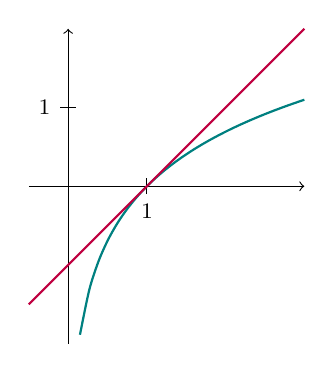
\begin{tikzpicture}
        \draw [->] (-0.5,0) -- (3,0);
        \draw [->] (0,-2) -- (0,2);
        \draw (1,-0.1) -- (1,0.1) node[below, yshift=-2mm] {\footnotesize $1$};
        \draw (-0.1,1) -- (0.1,1) node[left, xshift=-2mm] {\footnotesize $1$};
        \draw[thick, domain=0.15:3, smooth, variable=\x, teal] plot ({\x}, {ln(\x)});
        \draw[thick, domain=-0.5:3, smooth, variable=\x, purple] plot ({\x}, {\x-1});
      \end{tikzpicture}
      \caption{$\ln$ en bleu et $y=x-1$ en violet.}
    \end{figure}
  \end{minipage}
\end{question_kholle}

\begin{question_kholle}{Limite en $0$ de $\displaystyle\frac{(1+x)^{\alpha}-1}{x}$ et de $\displaystyle\frac{1-\cos x}{x^2}$.}
  \hfill
  \begin{itemize}[label=$*$]
    \item Le taux d'accroissement en $x_0$ d'une fonction $f$ dérivable en $x_0$ est
          \[\tag{$\star$}
            \lim_{x\to x_0}\frac{f(x)-f(x_0)}{x-x_0}=f'(x_0)
          \]
          \begin{itemize}
            \item En appliquant $(\star)$ pour $f\leftarrow \bigl(x\mapsto (1+x)^{\alpha}\bigr)$ et $x_0\leftarrow 0$, on a
                  \[
                    \lim_{x\to 0}\frac{f(x)-f(0)}{x-0}=\lim_{x\to x_0}\frac{(1+x)^{\alpha}-(1+0)^{\alpha}}{x-0} = \lim_{x\to 0}\frac{(1+x)^{\alpha}-1}{x}=f'(0)=\alpha
                  \]
                  car $f': x\mapsto 1\cdot \alpha\cdot (1+x)^{\alpha - 1}$ vaut $\alpha$ en $0$.
            \item De même, en appliquant $(\star)$ pour $f\leftarrow \sin$ et $x_0\leftarrow 0$, on a
                  \[
                    \lim_{x\to 0}\frac{f(x)-f(0)}{x-0}=\lim_{x\to x_0}\frac{\sin x-\sin 0}{x-0} = \lim_{x\to 0}\frac{\sin x}{x}=\sin' 0=\cos 0=1
                  \]
          \end{itemize}
    \item Soit $x\in\R^*$ fixé quelconque.
          \[
            \frac{1 - \cos x}{x^2} = \frac{(1-\cos x)(1+\cos x)}{x^2(1+\cos x)} = \frac{1-\cos^2 x}{x^2(1+\cos x)}=\biggl(\!\!\!\smash{\underbrace{\frac{\sin x}{x}}_{\arrowlim{x}{0}1}}\!\!\!\biggr)^2\cdot\underbrace{\left(\frac{1}{1+\cos x}\right)}_{\arrowlim{x}{0}\frac{1}{2}} \arrowlim{x}{0}\frac{1}{2}
          \]
  \end{itemize}
\end{question_kholle}

\begin{question_kholle}{Présentation exhaustive de la fonction $\arcsin$.}
  Premièrement, ladite fonction est la bijection réciproque de la fonction $\bigl.\sin\bigr|_{\left[ -\frac{\pi}{2}, \frac{\pi}{2}\right]}^{[-1,1]}$ (voir \textbf{1}.). D'où :
  \begin{equation*}
    \arcsin = \left\{
    \begin{array}{c c c}
      [-1,1] & \to     & [-\frac{\pi}{2} , \frac{\pi}{2}]                                                             \\ [1ex]
      x      & \mapsto & \left(\bigl.\sin\bigr|_{\left[ -\frac{\pi}{2}, \frac{\pi}{2}\right]}^{[-1,1]}\right)^{-1}(x)
    \end{array}
    \right.
  \end{equation*}
  Ainsi, pour $x\in [-1,1]$, $\arcsin (x)$ est l'unique solution de l'équation d'inconnue $\theta \in \textstyle \left[-\frac{\pi}{2} , \frac{\pi}{2}\right]$ :
  \[
    \sin(\theta) = x
  \]
  .
  \noindent Il découle alors naturellement des propriétés héréditairement acquises de $\bigl.\sin\bigr|_{\left[ -\frac{\pi}{2}, \frac{\pi}{2}\right]}^{[-1,1]}$ :

  \begin{enumerate}
    \item $\arcsin$ est impaire.
    \item $\arcsin$ est strictement croissante sur $[-1,1]$.
    \item $\arcsin \in \mathcal{C}^0\left([-1,1],[-\frac{\pi}{2} , \frac{\pi}{2}] \right)$.
    \item $\arcsin \in \mathcal{D}^1\left(]-1,1[,\left]-\frac{\pi}{2} , \frac{\pi}{2}\right[ \right)$.
    \item $\arcsin'(x) = \frac{1}{\sqrt{1-x^2}}$ pour tout $x\in]-1,1[$.
    \item $\arcsin$ admet deux demi-tangentes verticales en $-1$ et $1$.
  \end{enumerate}

  \

  Graphe de $\arcsin$ :
  \begin{figure}[H]
    \centering
    \begin{tikzpicture}[scale=2]
      \draw [->] (-1.5,0) -- (1.5,0);
      \draw [->] (0,-pi/2-0.5) -- (0,pi/2+0.5);
      \draw (1,-0.05) -- (1,0.05) node[below, yshift=-3mm] {\footnotesize $1$};
      \draw (-0.05,pi/2) -- (0.05,pi/2) node[left, xshift=-3mm] {\footnotesize $\frac{\pi}{2}$};
      \draw[thick, domain=-1.5:1.5, smooth, variable=\x, lime] plot ({\x}, {sin(\x*180/pi)});
      \draw[thick, domain=-1.5:1.5, smooth, variable=\x, teal] plot ({\x}, {\x});
      \draw[thick, domain=-1:1, samples=100, variable=\x, purple] plot ({\x}, {pi*asin(\x)/180});
      \draw [->] (-1,-pi/2) -- (-1,-pi/2+0.5);
      \draw [->] (1,pi/2) -- (1,pi/2-0.5);
      \draw [->] (pi/2,1) -- (pi/2-0.5,1);
      \draw [->] (-pi/2,-1) -- (-pi/2+0.5,-1);
    \end{tikzpicture}
    \caption{$\arcsin$ en violet, $\sin$ en vert et la première bissectrice en bleu.}
  \end{figure}
  On a aussi, grâce au taux d'accroissement en 0 d'$\arcsin$ :
  \[
    \lim_{x\to0} \frac{\arcsin(x)}{x} \ = \ 1.
  \]

  \

  Puis finalement (visible sur le graphe) :
  \[
    \forall x \in [0,1], \quad \arcsin(x) \geq x.
  \]
\end{question_kholle}

\begin{question_kholle}{Étude et tracé de $\arcsin\circ\sin$ (avec réduction du domaine d'étude à $[0,\pi/2]$).}\hfill
  \begin{itemize}[label=$*$]
    \item La fonction $\sin$ est définie sur $\R$ et $\sin(\R)=[-1,1] = \mathcal{D}_{\arcsin}$ donc $\arcsin\circ\sin$ est définie sur $\R$.
    \item La fonction $\arcsin\circ\sin$ est $2\pi$-périodique car $\sin$ est $2\pi$-périodique. On peut donc restreindre le domaine d'étude à un intervalle d'amplitude $2\pi$, par exemple $[-\pi,\pi]$.
    \item La fonction $\arcsin\circ\sin$ est impaire comme composée de fonctions impaires. L'intervalle $[-\pi,\pi]$ étant centré en $0$, on peut restreindre le domaine d'étude à $[0,\pi]$.
    \item De plus, pour tout $x\in [0,\pi]$, $\sin(\pi - x)=\sin x$ donc $(\arcsin\circ\sin)(\pi-x)=(\arcsin\circ\sin)(x)$ .
  \end{itemize}
  Il suffit donc d'étudier le graphe fonction $\arcsin\circ\sin$ sur l'intervalle $\left[0,\frac{\pi}{2}\right]$, son graphe sur $[0,\pi]$ s'en déduisant par une réflexion d'axe la droite d'équation $x=\frac{\pi}{2}$, ce qui nous permet, par imparité et $2\pi$-périodicité, de trouver son graphe sur $\R$ par réflexion sur l'axe des ordonnées et translations successives de vecteur $2\pi\vv{i}$.\\
  Sachant que pour tout $x\in\left[0,\frac{\pi}{2}\right], (\arcsin\circ\sin)(x) = x$, on a le graphe suivant~:

  \begin{figure}[H]
    \centering
    \begin{tikzpicture}[scale=1.5]
      \draw [->] (-3*pi/2,0) -- (3*pi/2,0);
      \draw [->] (0,-pi/2-0.5) -- (0,pi/2+0.5);
      \draw [dashed] (pi/2,-pi/2-0.5) -- (pi/2,pi/2+0.5);
      \draw [thick, ->] (0,0) -- (1,0) node[midway, below] {$\vv{i}$};

      % Graduations
      \draw (pi/2,-0.05) -- (pi/2,0.05) node[below, yshift=-3mm, fill=white] {\footnotesize $\frac{\pi}{2}$};
      \draw (pi,-0.05) -- (pi,0.05) node[below, yshift=-3mm] {\footnotesize $\pi$};
      \draw (-0.05,pi/2) -- (0.05,pi/2) node[left, xshift=-3mm] {\footnotesize $\frac{\pi}{2}$};

      % Courbes
      \draw[thick, dashed, domain=-3*pi/2:-3*pi/2+0.3, variable=\x, gray] plot ({\x}, {pi*asin(sin(\x*180/pi))/180});
      \draw[thick, dashed, domain=3*pi/2-0.3:3*pi/2, variable=\x, gray] plot ({\x}, {pi*asin(sin(\x*180/pi))/180});
      \draw[thick, domain=-3*pi/2+0.3:3*pi/2-0.3, samples=100, variable=\x, gray] plot ({\x}, {pi*asin(sin(\x*180/pi))/180});
      \draw[thick, domain=0:pi/2, variable=\x, purple] plot ({\x}, {pi*asin(sin(\x*180/pi))/180});
      \draw[thick, domain=pi/2:pi, variable=\x, teal] plot ({\x}, {pi*asin(sin(\x*180/pi))/180});
      \draw[thick, domain=-pi:0, variable=\x, lime] plot ({\x}, {pi*asin(sin(\x*180/pi))/180});
    \end{tikzpicture}
    \caption{Graphe de $\arcsin\circ\sin$.}
  \end{figure}
\end{question_kholle}
\end{document}
